\subsubsection{Validierung des Algorithmus durch Testläufe}
\label{chap:Validierung des Algorithmus durch Testläufe}

Zuerst werden einige Durchläufe des bereits implementierten Netzwerks mit drei Neuronen durchgeführt. Als Hyperparameter werden \(\beta=1\) und \(\eta=0.5\) definiert, jeweils die Ausgaben zweier Durchläufe des \gls{c-ep} sind in Abbildung \ref{fig:C-EP Sim 1,2} dargestellt. Alle hier aufgeführten Simulationen werden mit 10 Zeiteinheiten für die freie und 10 für die feste Phase durchgeführt, was einer Dauer von 20 Zeiteinheiten pro Epoche entspricht. In Abbildung \ref{fig:C-EP Sim 1,2} sind zwei Durchläufe des Lernprozesses mit den genannten Hyperparametern dargestellt. Die Zielwerte \(\vec{d}=(0.3,0.8,0.5)\) findet das \gls{c-ep} innerhalb von ca. 1700 Zeiteinheiten, was 85 Epochen entspricht. Kurz nachdem die Zielwerte erreicht und die Kostenfunktion damit minimiert wurde, wurden die Gewichtsanpassungen chaotisch. Die zweite Simulation mit \(\vec{d}=(0,1,0)\) zeigt, dass sich das Netzwerk an die Grenzwerte \(0,1\) zwar annähert, diese aber nicht ohne größeren Fehler erreicht.

\begin{figure}[h]
  \centering
  \begin{subfigure}[b]{0.5\textwidth}
    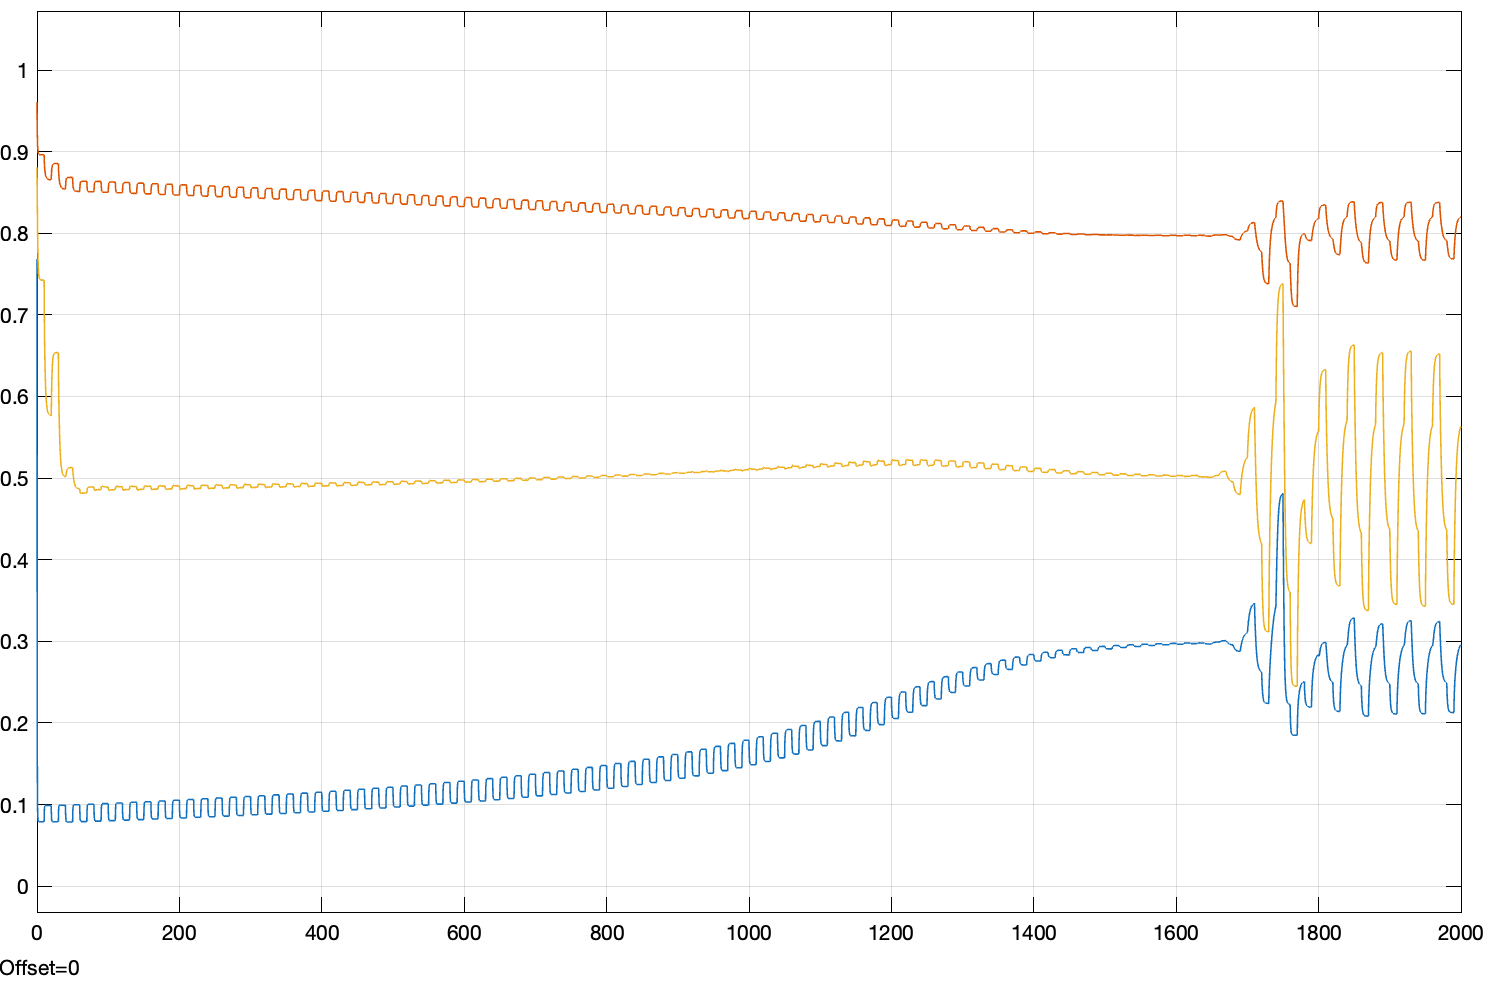
\includegraphics[width=\textwidth]{abbildungen/c_ep_sim_1_ausgabe.png}
    \caption{\(\vec{d}=(0.3,0.8,0.5)\)}
  \end{subfigure}%
  \hfill
  \begin{subfigure}[b]{0.5\textwidth}
    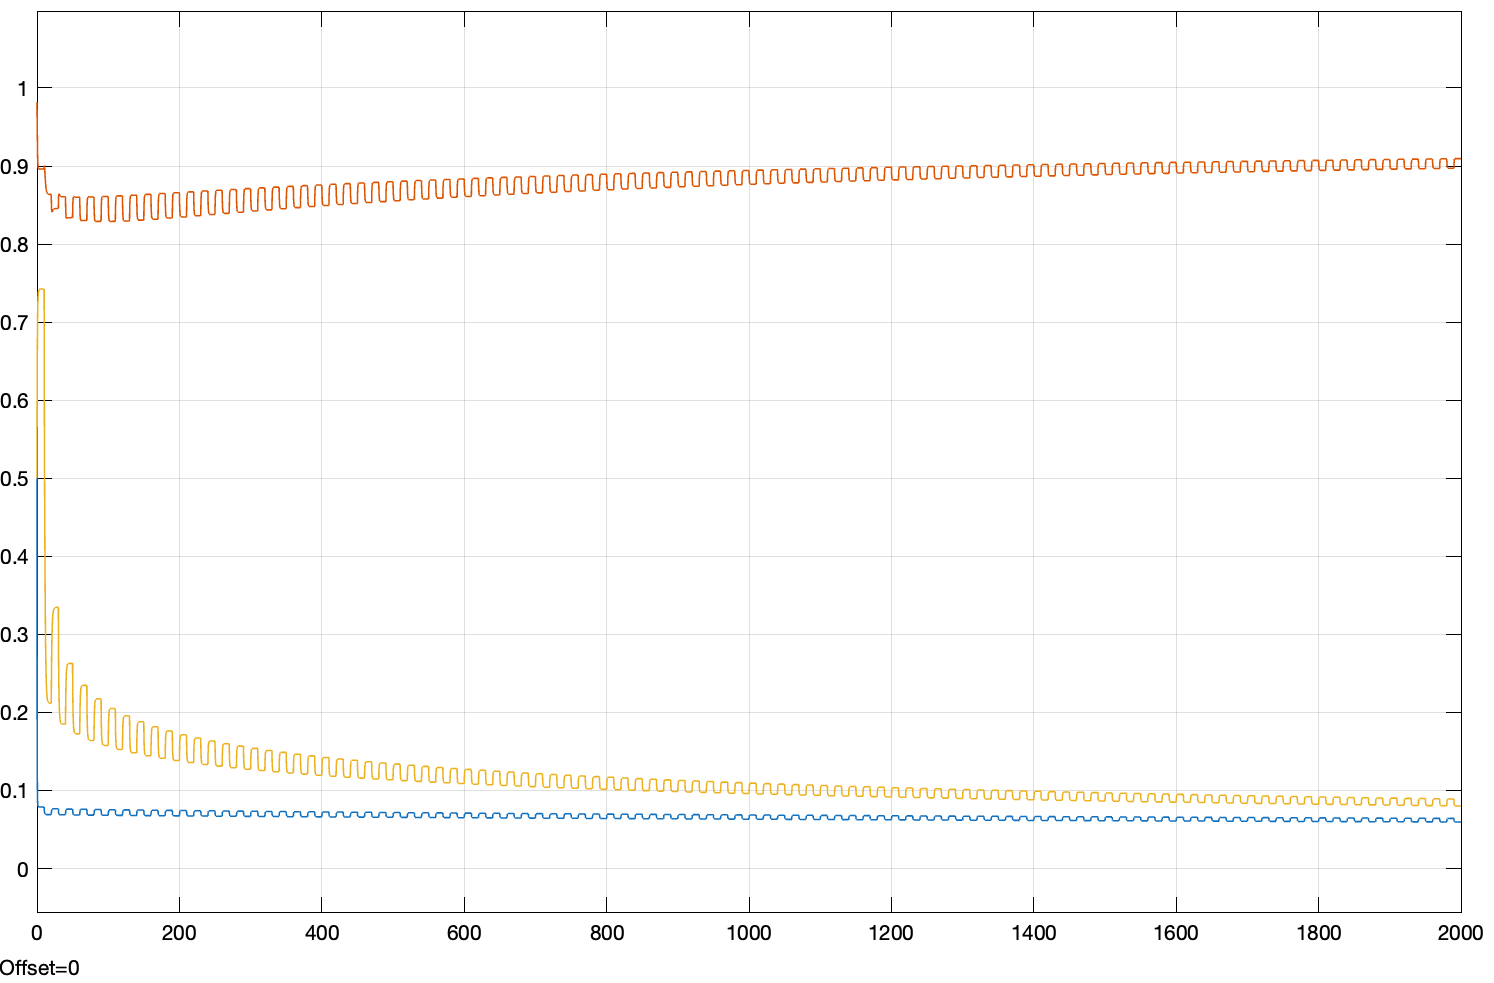
\includegraphics[width=\textwidth]{abbildungen/c_ep_sim_2_ausgabe.png}
    \caption{\(\vec{d}=(0,1,0)\)}
  \end{subfigure}
  \caption{Simulationen des \gls{c-ep} mit \(\beta=1,\eta=0.5\). Dargestellt ist die Ausgabe des Netzwerks. Quelle: \textit{Eigene Darstellung}}
  \label{fig:C-EP Sim 1,2}
\end{figure}

In Abbildung \ref{fig:C-EP Sim 5} ist diese Annäherung erneut dargestellt, diesmal mit den extremen Hyperparametern \(\eta=10,\beta=1\). Zu sehen ist, dass sich das Netzwerk auf nahezu \(0\) annähert, dies aber in einer nicht trivialen Weise, da ein so groß gewähltes \(\eta\) die Konvergenz für Zielwerte \(0<d<1\) erschwert. Der Lernprozess wurde auch für \(\vec{d}=(-1,-1,-1)\) und \(\vec{d}=(2,2,2)\) durchgeführt, mit diesen Zielwerten nähert sich die Ausgabe des Netzwerk \(0\) bzw. \(1\).

\begin{figure}[h]
  \centering
  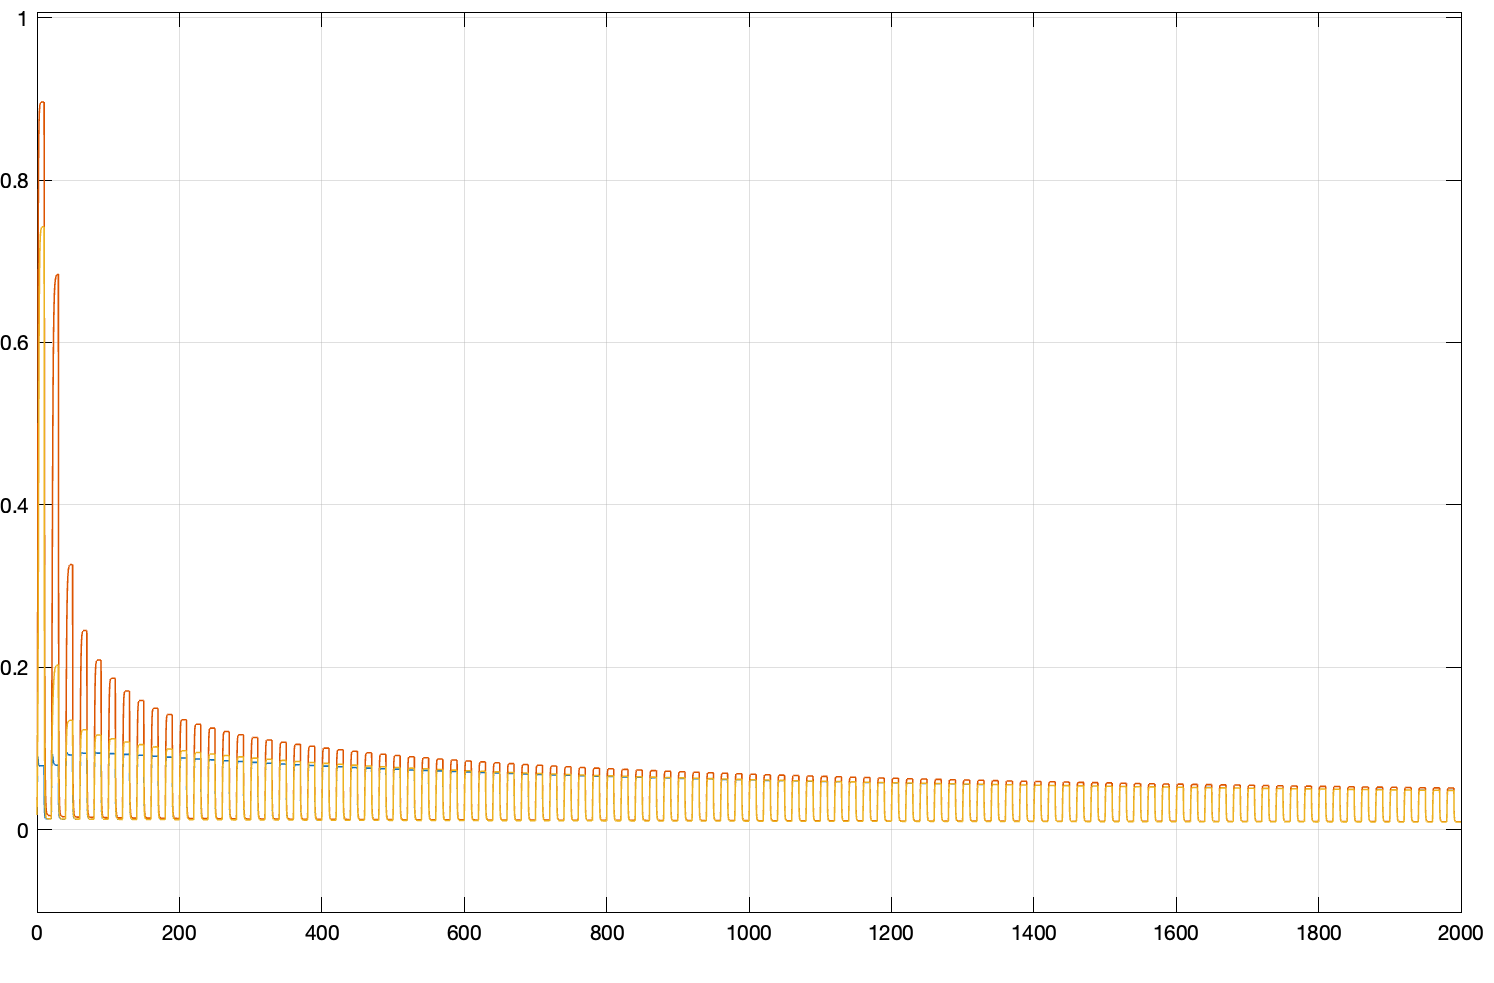
\includegraphics[width=0.5\textwidth]{abbildungen/c_ep_sim_5_ausgabe.png}
  \caption{Annäherungen des \gls{c-ep} an den Grenzwert \(0\). Quelle: \textit{Eigene Darstellung}}
  \label{fig:C-EP Sim 5}
\end{figure}

Das \gls{c-ep} wurde auch mit einer alternativen Aktivierungsfunktion \(tanh(x)=\frac{e^x-e^{-x}}{e^x+e^{-x}}\) und den Zielwerten \((-1,-1,1)\) simuliert. Die Besonderheit dieser Funktion im Vergleich zur bisher genutzten logistischen Funktion ist der Wertebereich \([-1;1]\). Damit lassen sich, wie in Abbildung \ref{fig:C-EP Sim 6} gezeigt, auch negative Zielwerte mit einem Fehler von \(C(y)\approx0.0067\) abbilden, wodurch andere Anwendungsfälle bedient werden können. Die gezeigten Simulationen wurden mit einer skalierten Variante der genannten Funktion durchgeführt \(\rho(x)=tanh(2x)\).

\begin{figure}[h]
  \centering
  \begin{subfigure}[b]{0.5\textwidth}
    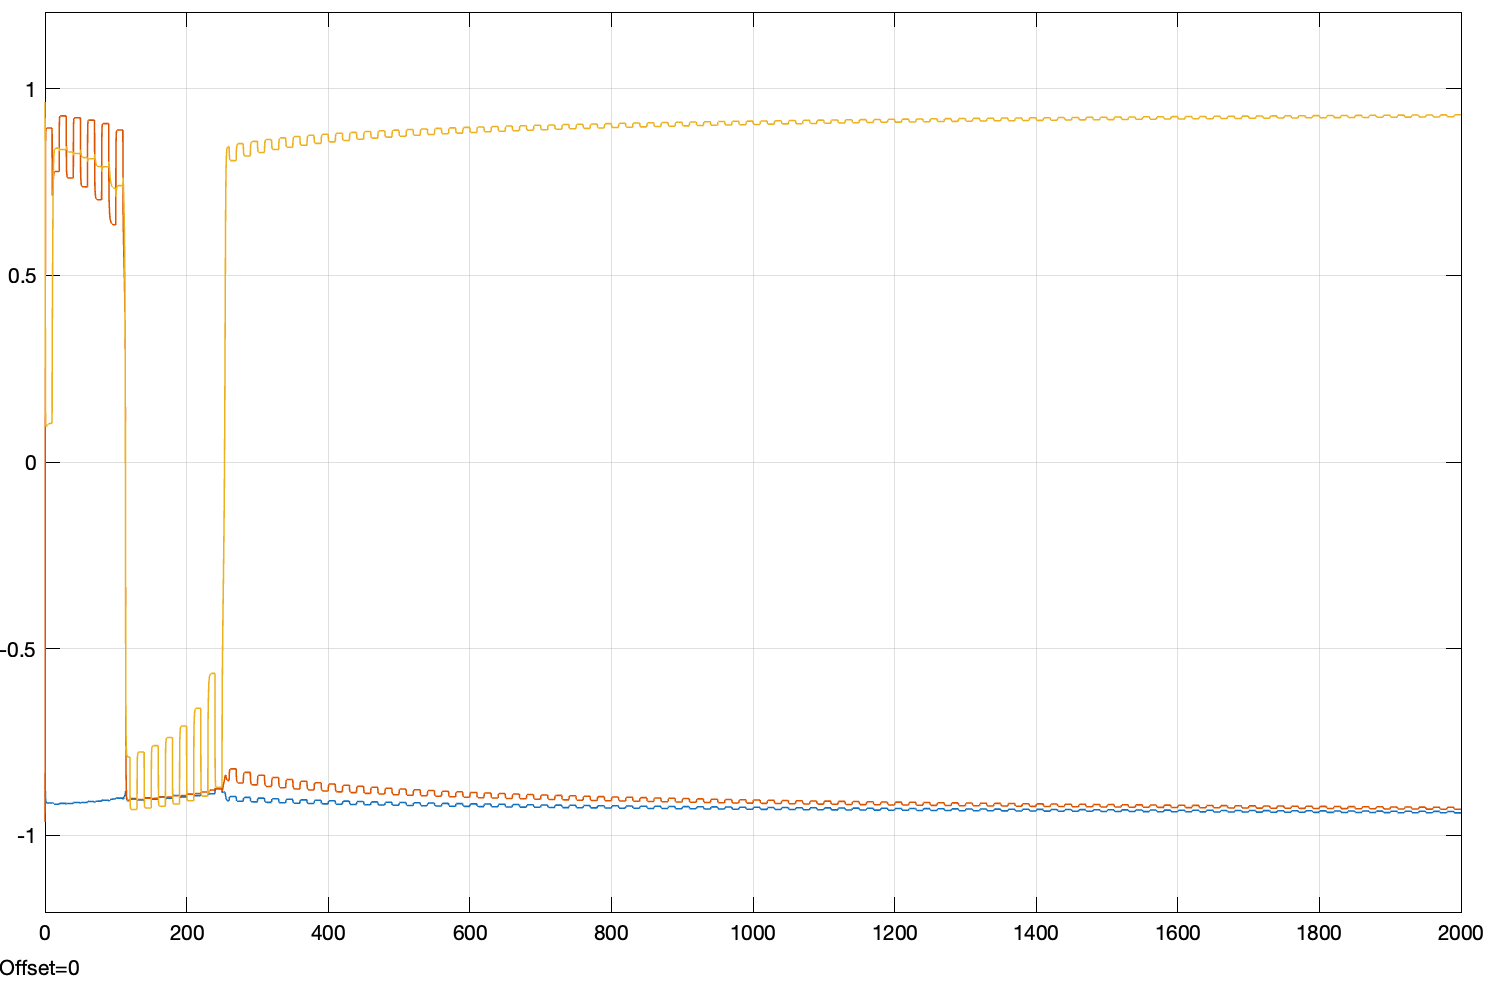
\includegraphics[width=\textwidth]{abbildungen/c_ep_sim_6_ausgabe.png}
    \caption{Ausgabe des Netzwerks}
  \end{subfigure}%
  \hfill
  \begin{subfigure}[b]{0.5\textwidth}
    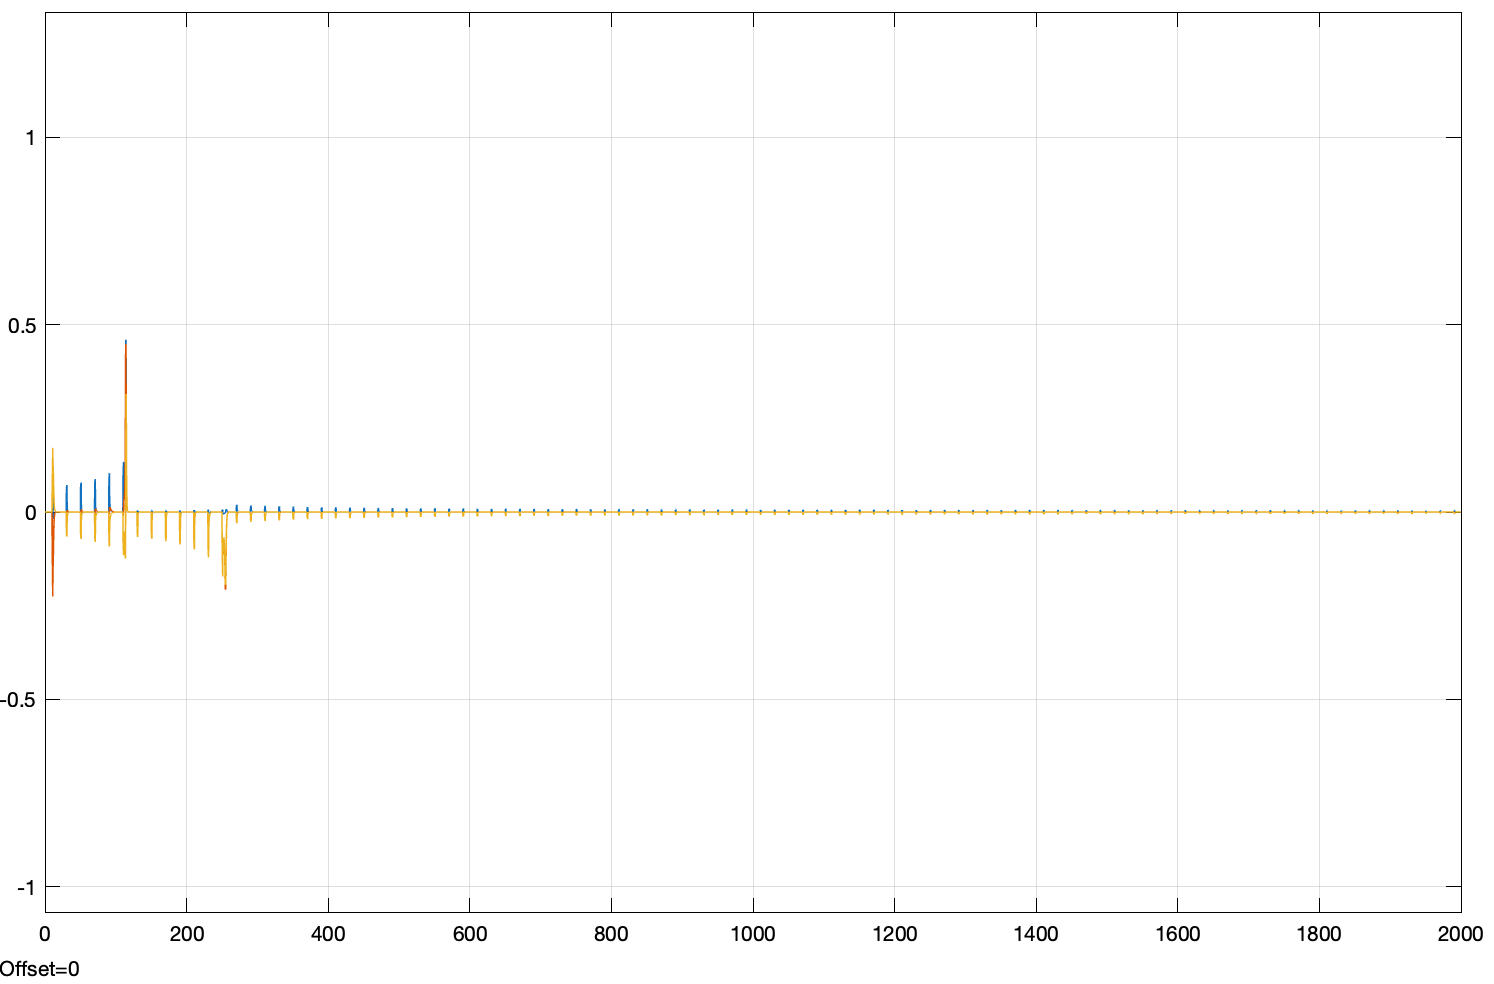
\includegraphics[width=\textwidth]{abbildungen/c_ep_sim_6_weight_update.png}
    \caption{Gewichtsanpassungen}
  \end{subfigure}
  \caption{Simulationen des \gls{c-ep} mit der Aktivierungsfunktion: \(\rho(x)=tanh(2x)\). Quelle: \textit{Eigene Darstellung}}
  \label{fig:C-EP Sim 6}
\end{figure}

Wie bereits im Kapitel \ref{chap:Strategien zur Fehlerbehebung und Optimierung} beschrieben, führt die Aktivierungsfunktion "`ReLU"' im Zusammenhang mit dem hier implementierten \gls{hopfieldnetzwerk} zu unerwarteten Fehlern. Der schlagartige Anstieg der Zustände des Netzwerks ist in Abbildung \ref{fig:C-EP Sim 7} dargestellt.

\begin{figure}[h]
  \centering
  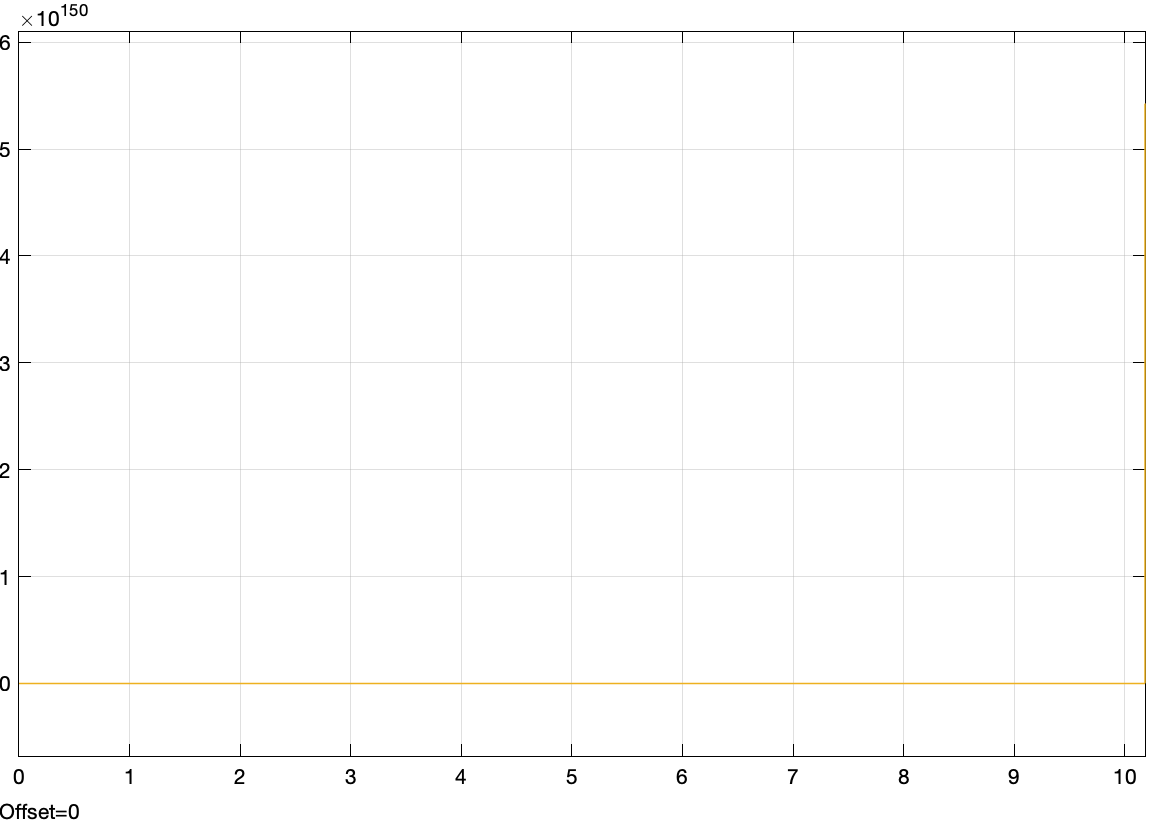
\includegraphics[width=0.5\textwidth]{abbildungen/c_ep_sim_7_state_dynamics.png}
  \caption{Simulation des \gls{c-ep} mit der Aktivierungsfunktion "`ReLU"' (\(R(x)=max(x,0)\)). Gezeigt wird die Dynamik der Zustände des Netzwerks \(\frac{ds}{dt}\). Quelle: \textit{Eigene Darstellung}}
  \label{fig:C-EP Sim 7}
\end{figure}

Ein fehlerfreies Speichern von \(N\) Mustern im \gls{hopfieldnetzwerk} erfordert eine Mindestanzahl von \(\frac{N}{0.15}\) Neuronen, was einer Anzahl von 14 Neuronen zum Speichern von zwei Mustern, 20 für drei Muster usw. entspricht \cite[vgl. S. 2556]{Hopfield1982}. In dieser Arbeit konnte bisher gezeigt werden, dass ein einziges Muster mit einem Netzwerk aus drei Neuronen mit einem Fehler unter \(0.1\) gespeichert werden kann. Die Konstruktion eines Netzwerks mit 14 (oder mehr) Neuronen erfordert aber eine überproportional komplexe Suche nach Hyperparametern für den Lernprozess, in Verbindung mit dem erforderlichen Rechenaufwand ist eine größere Simulation sehr unattraktiv. Aus diesem Grund wurde das Modell nur auf eine Größe von sechs Neuronen erweitert und so auf die Zielwerte \(\vec{d}=(0.3,0.6,0.3,0.8,0.8,0.8)\) trainiert, siehe Abbildung \ref{fig:C-EP Sim 3}. Die für die Simulation gefundenen Hyperparameter lauten \(\eta=0.05,\beta=0.5\), die Simulation wurde für 10.000 Zeiteinheiten, also 500 Epochen, durchgeführt. Damit erreicht das Netzwerk einen Fehler von \(C(y)\approx0.0709\).

\begin{figure}[h]
  \centering
  \begin{subfigure}[b]{0.5\textwidth}
    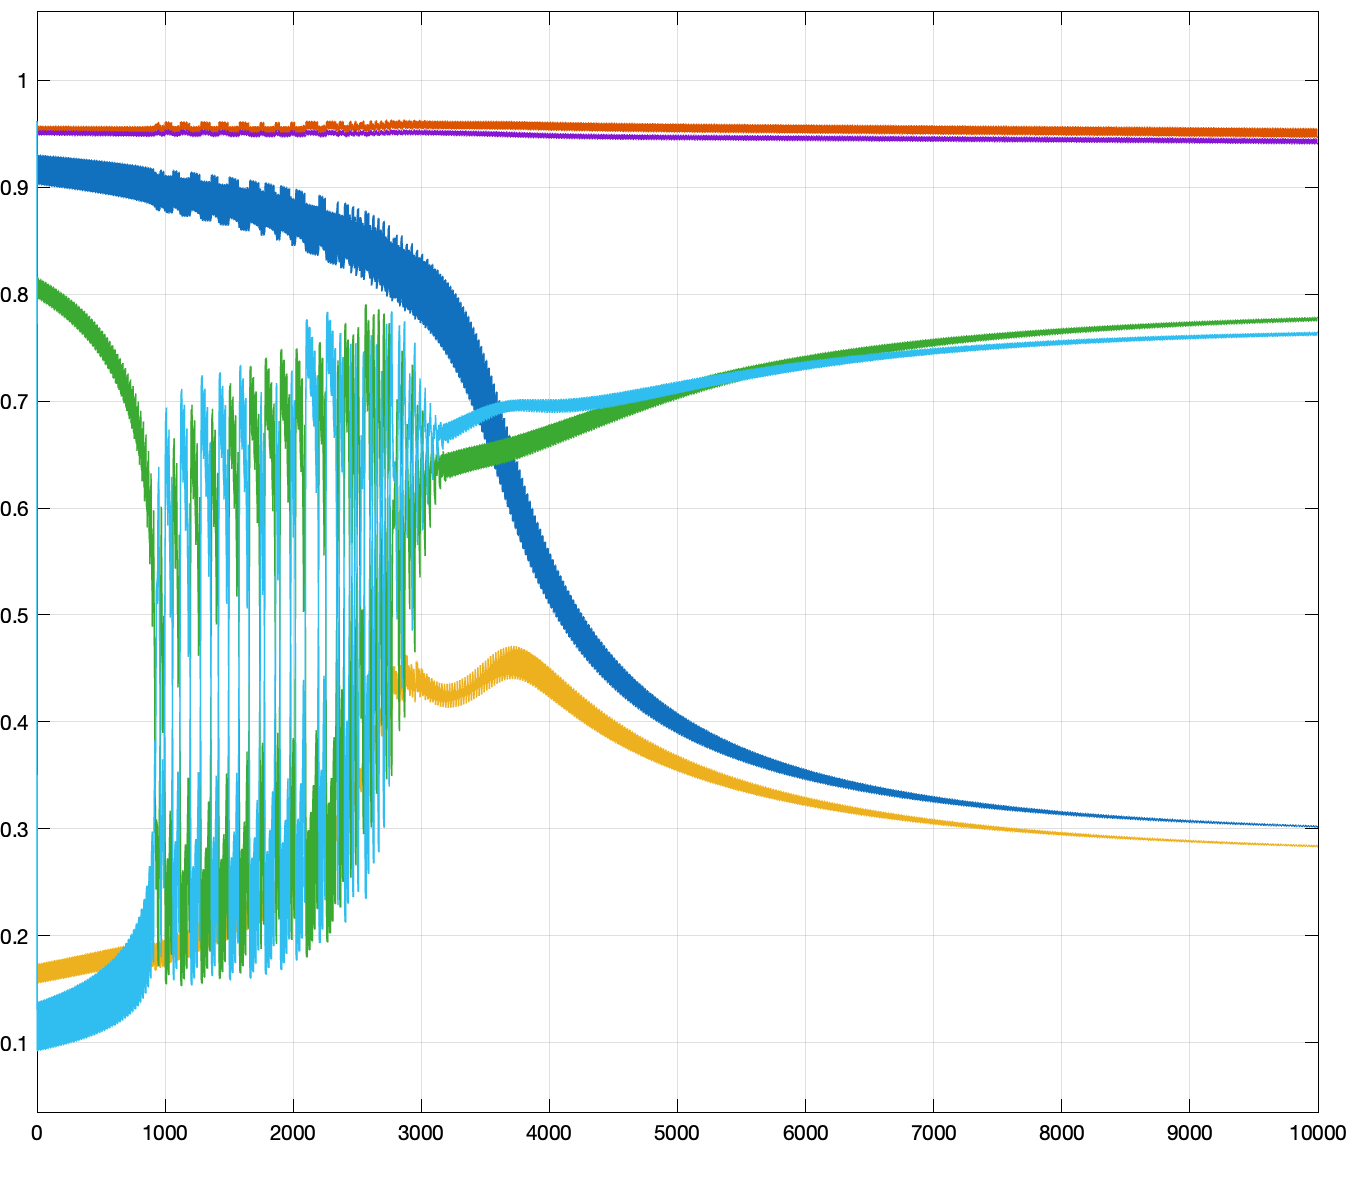
\includegraphics[width=\textwidth]{abbildungen/c_ep_sim_3_ausgabe.png}
    \caption{Ausgabe des Netzwerks}
  \end{subfigure}%
  \hfill
  \begin{subfigure}[b]{0.5\textwidth}
    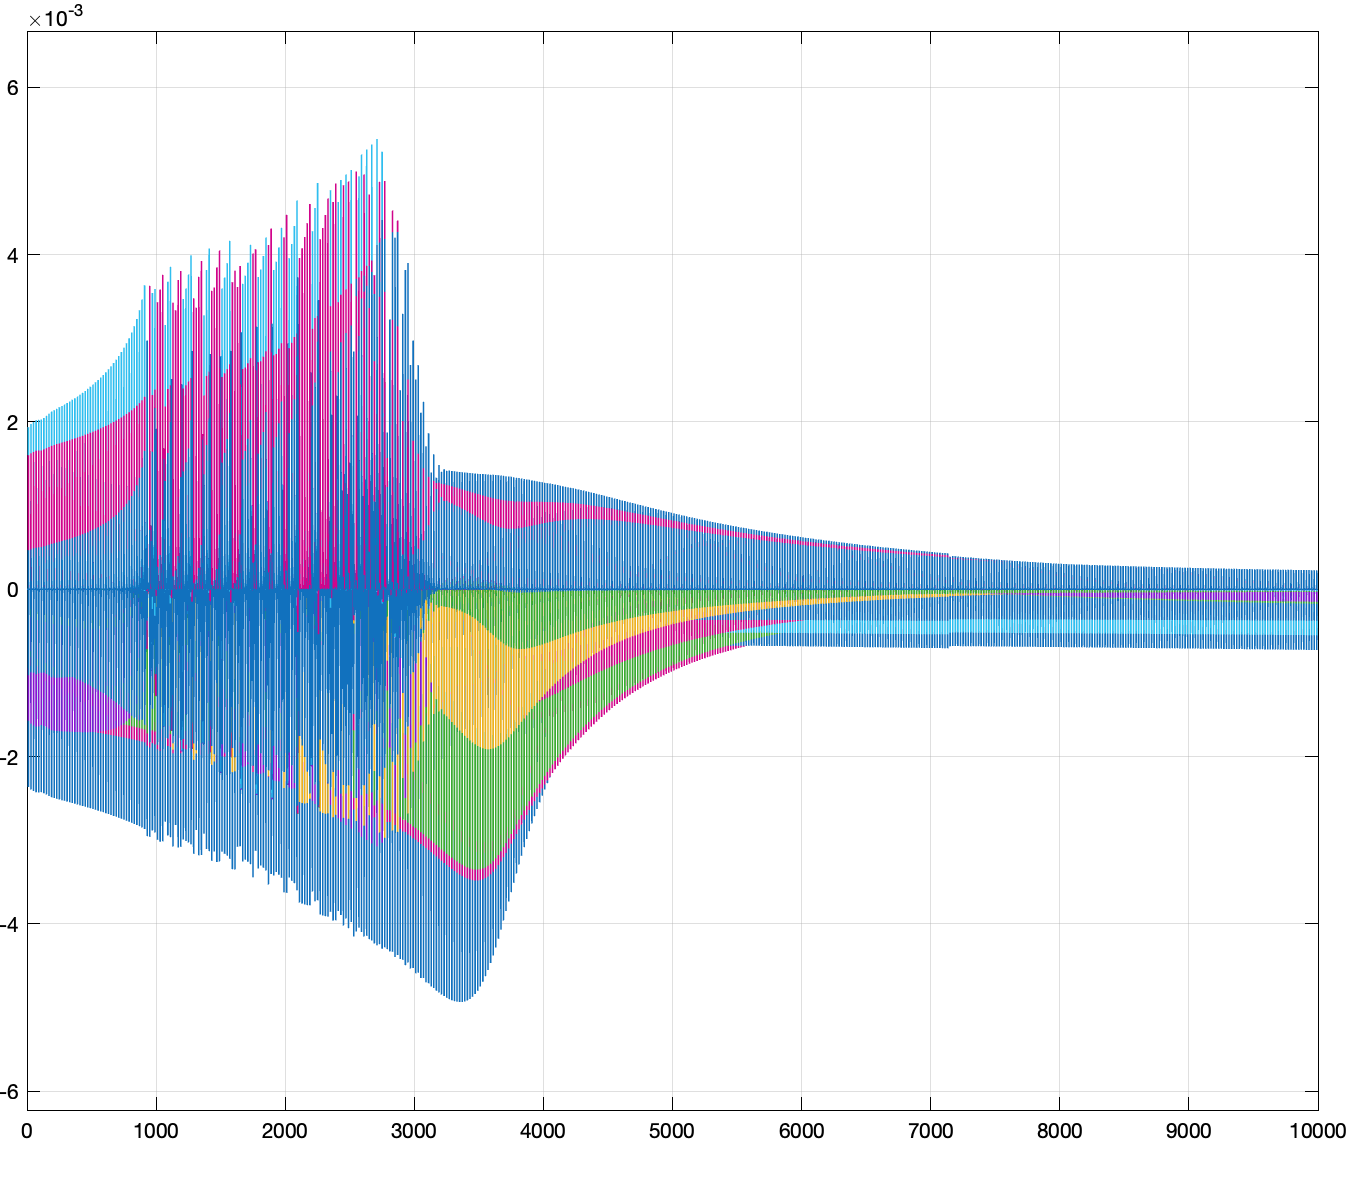
\includegraphics[width=\textwidth]{abbildungen/c_ep_sim_3_weight_update.png}
    \caption{Gewichtsanpassungen}
  \end{subfigure}
  \caption{Simulationen des \gls{c-ep} mit 6 Neuronen. Quelle: \textit{Eigene Darstellung}}
  \label{fig:C-EP Sim 3}
\end{figure}
